%EMPIRICAL STUDY
In this section, we experimentally study the performance of our proposed algorithms through comprehensive experiments on both real and synthetic datasets. We describe the experimental settings in Section 6.1, and report the performance of our proposed algorithms for KaGWC queries on synthetic and real datasets in Sections 6.2 and 6.3 respectively.

\subsection{Experimental Setup}
\textbf{Algorithms.} We evaluate the performance of the following proposed algorithms: the approximation algorithm CubeTree in Section 5.1, the approximation algorithm MaxMargin in Section 5.2, and the exact algorithm MergeList in Section 5.3.

\textbf{Data and queries.} We conduct experiments with two datasets, namely synthetic dataset and real-life dataset. Our experiments were carried out primarily on synthetic dataset with five major factors, namely, 1) \textit{the total number of keywords in the spatial object database} (TK), 2) \textit{data size} (DS), 3) \textit{the number of query keywords} (QK), 4) \textit{the upper bound of the number of keywords associated with each object} (KD), not the fixed number of keywords in \cite{zhang2009keyword}, 5) \textit{the weight constraint threshold of query q} (TS). We study their effect on both response time and approximation ratio in three algorithms. Synthetic data generator generates three types of datasets following the uniform, random and zipf (URZ) distribution respectively. For each query, we repeat 5 times experiment for each type of dataset. We also included real dataset CA, which was collected from the U.S. Board on Geographic Names(geonames.usgs.gov). For each query, we repeat 10 times experiment.

All three algorithms were implemented in C/C++ and run on an Intel(R) Core(TM)2 Quad CPU Q8400 @2.66Hz with 4GB RAM.

\subsection{Results on Synthetic Dataset}
To measure the comprehensive performance of our algorithms on different types of datasets, in this section, we employ the URZ average response time $(URZA\_T)$ and URZ average approximation ratio $(URZA\_R)$ as the measurements, where $URZA\_T=\frac{T_u+T_r+T_z}{3}, URZA\_R=\frac{R_u+R_r+R_z}{3}$. $Tu, Tr, Tz$ and $Ru, Rr, Rz$ represent the response time and approximation ratio of uniform, random and zipf distribution datasets, respectively. Table \ref{T6} illustrates all the possible values for these factors in subsequent experiments. Note that, we use bold font to denote the default value for each factor. We repeat query 5 times for each dataset, and we take the average value of all datasets as the final result.

\begin{table}[h]
\centering
\begin{tabular}{|l|l|}
\hline
Factors & Instance Value \\
\hline
TK & 50,100,150,200,250,\textbf{300} \\
\hline
DS($10^4$) & 1,\textbf{10},30,50,70,90\\
\hline
QK & 2,\textbf{3},4,5,6,7,8,9 \\
\hline
KD & 3,5,\textbf{7},9,11,13,15 \\
\hline
TS & 0.1,\textbf{0.2},0.3,0.4,0.5,0.6,0.7 \\
\hline
\end{tabular}
\caption{The real data of CA}
\label{T6}
\end{table}

\begin{figure}[h] \centering
    \subfigure[] { \label{TKa}
    \includegraphics[width=1.5in,height=1.5in]{TK-T}
    }
    \subfigure[] { \label{TKb}
    \includegraphics[width=1.5in,height=1.5in]{TK-R}
    }
\caption{Varying the factor TK}
\label{F4}
\end{figure}

\textbf{\textit{Varying the factor TK}}. Figs. \ref{F4}a and \ref{F4}b show the response time and approximation ratio of three algorithms respectively, when we vary the value of TK. As shown in Fig. \ref{F4}a, the response time of MergeList decreases dramatically as TK becomes larger. CubeTree runs faster than does MaxMargin. And both CubeTree and MaxMargin decrease slightly as TK is increased. The reason behind is that, when other factors are fixed, the larger the TK, the smaller number of relevant objects, and thus smaller objects need to be handled during algorithms execution. It is also denoted that MergeList is more sensitive than CubeTree and MaxMargin in terms of TK. In Fig. \ref{F4}b, we set the approximation ratio of the exact algorithm MergeList equals to 1, which is also adopted by the subsequent experiments. It can be observed from Fig. \ref{F4}b that, MaxMargin achieves a much better accuracy than CubeTree. And the approximation ratio of MaxMargin changes slightly and with an upper bound 1.25 when we vary the value of TK. In contrast, the approximation ratio of CubeTree changes dramatically and with an upper bound 3.5. This is because MaxMargin always select the optimal object and update the contribution ratio dynamically.

\begin{figure}[h] \centering
    \subfigure[] { \label{DSa}
    \includegraphics[width=1.5in,height=1.5in]{DS-T}
    }
    \subfigure[] { \label{DSb}
    \includegraphics[width=1.5in,height=1.5in]{DS-R}
    }
\caption{Varying the factor DS}
\label{F5}
\end{figure}

\textbf{\textit{Varying the factor DS}}. Figs. \ref{F5}a and \ref{F5}b show the response time and approximation ratio of three algorithms respectively, when we vary the value of DS. We vary the value of DS from 10,000 to 900,000. As expected, as DS increases, the response time of all three algorithms increase. However, as shown in the Fig. \ref{F5}a, the response time of MergeList does not increase dramatically as DS is increased. This is due to the two pruning strategies Lemma 3 and Lemma 4 employed in MergeList. Specifically, although CubeTree runs faster than MaxMargin but the response time of MaxMargin increases slowly than CubeTree in that the merge phase takes much time when DS increases, which reflects that MaxMargin is more adaptive to DS than CubeTree. Fig. \ref{F5}b shows MaxMargin achieves an approximation ratio from 1.0 to 1.2 when we vary DS from 10,000 to 900,000. Especially, the approximation ratio equals to 1 when DS takes the value of 300,000. The approximation ratio of CubeTree with an upper bound 2.0, however, it is unstable.

\begin{figure}[h] \centering
    \subfigure[] { \label{QKa}
    \includegraphics[width=1.5in,height=1.5in]{QK-T}
    }
    \subfigure[] { \label{QKb}
    \includegraphics[width=1.5in,height=1.5in]{QK-R}
    }
\caption{Varying the factor QK}
\label{F6}
\end{figure}

\textbf{\textit{Varying the factor QK}}. Figs. \ref{F6}a and \ref{F6}b show the response time and approximation ratio of three algorithms respectively, when we vary the value of QK. In this experiment, we vary the value of QK from 2 to 9. We omit the experiment results when MergeList runs out of memory (e.g., we omit the response time of MergeList in Fig. \ref{F6}a when QK takes the value of 7, 8 and 9, in that it runs out of memory). As shown in Fig. \ref{F6}a, MaxMargin and CubeTree run faster than MergeList. Usually, they are 7-20 times faster than MergeList and their response times are almost not affected by QK as shown in Fig. \ref{F6}a. This is because that with the KHT index, CubeTree can merge the cubeTree nodes efficiently and MaxMargin can select the optimal object from KMPQ directly. Since the exact algorithm MergeList fails to return the optimal solution when QK takes value of 7, 8 and 9, to maintain the integrity of the experiment result curve, for approximation algorithm CubeTree and MaxMargin, we take the average value of existing approximation ratio as the default value. We present these values with the dotted line in Fig. \ref{F6}b. These strategies used in this part also be used in subsequent experiments. As can be observed from Fig. \ref{F6}b, MaxMargin still achieves a better accuracy than CubeTree.

\begin{figure}[h] \centering
    \subfigure[] { \label{KDa}
    \includegraphics[width=1.5in,height=1.5in]{KD-T}
    }
    \subfigure[] { \label{KDb}
    \includegraphics[width=1.5in,height=1.5in]{KD-R}
    }
\caption{Varying the factor KD}
\label{F7}
\end{figure}

\textbf{\textit{Varying the factor KD}}. Figs. \ref{F7}a and \ref{F7}b show the response time and approximation ratio of three algorithms respectively, when we vary the value of KD. Differing with the method in \cite{zhang2009keyword}, which fixes the number of keywords associated with objects, in this set of experiments, we set the upper bound for it by KD. For each object, k keywords are generated, where k is a random positive integer less than the upper bound. We vary KD from 3 to 15. It is shown that MaxMargin and CubeTree run much faster than MergeList as the increases of KD. Specifically, we notice that the response time of all three algorithms increases as KD becomes larger. This is because that the number of relevant objects increases as KD increases. Fig. \ref{F7}b shows that the approximation ratio of MaxMargin changes slightly and is extremely close to 1. In contrast, CubeTree performs the worst in terms of accuracy and stability.

\begin{figure}[h] \centering
    \subfigure[] { \label{TSa}
    \includegraphics[width=1.5in,height=1.5in]{TS-T}
    }
    \subfigure[] { \label{TSb}
    \includegraphics[width=1.5in,height=1.5in]{TS-R}
    }
\caption{Varying the factor TS}
\label{F8}
\end{figure}

\textbf{\textit{Varying the factor TS}}. Figs. \ref{F8}a and \ref{F8}b show the response time and approximation ratio of three algorithms respectively, when we vary the value of TS. The value of TS determines the size of result set, besides, we can obtain the different combinations of object by adjusting TS. In this set of experiments, we vary TS from 0.1 to 0.7. As can be seen from Fig. \ref{F8}a that the response time of MergeList increases dramatically. Especially, MergeList runs out of memory when TS takes the value of 0.6. In contrast, CubeTree and MaxMargin are more adaptive to TS and almost not affected by TS as shown in Fig. \ref{F8}a. This is consistent with earlier findings when we study on the factor of QK. And can be explained with the same reason. Fig. \ref{F8}b shows again, that MaxMargin performs better than CubeTree in terms of approximation ratio.


\begin{figure}[h] \centering
    \subfigure[] { \label{CubeTree-T}
    \includegraphics[width=1.5in,height=1.5in]{CubeTree-T}
    }
    \subfigure[] { \label{MaxMargin-T}
    \includegraphics[width=1.5in,height=1.5in]{MaxMargin-T}
    }
    \subfigure[] { \label{MergeList-T}
    \includegraphics[width=1.5in,height=1.5in]{MergeList-T}
    }
\caption{The Response Time on Different Datasets}
\label{F11}
\end{figure}

\begin{figure}[!ht] \centering
    \subfigure[] { \label{CubeTree-R}
    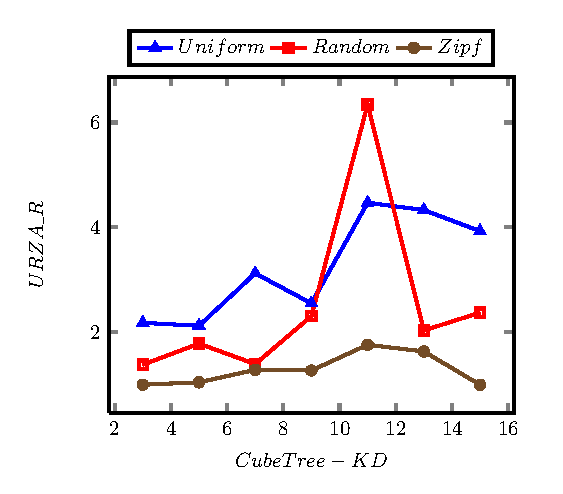
\includegraphics[width=1.5in,height=1.5in]{CubeTree-R}
    }
    \subfigure[] { \label{MaxMargin-R}
    \includegraphics[width=1.5in,height=1.5in]{MaxMargin-R}
    }
    \subfigure[] { \label{MergeList-R}
    \includegraphics[width=1.5in,height=1.5in]{MergeList-R}
    }
\caption{The Approximation Ratio on Different Datasets}
\label{F12}
\end{figure}

\textbf{\textit{The performance on Different Datasets.}} To further illustrate the performance of our algorithms on different types of datasets. In this set of experiments, we study the performance of our proposed algorithms on different datasets from the aspect of KD. Figs. \ref{F11} and \ref{F12} show the response time and approximation ratio of our algorithms on different datasets, respectively. Specifically, Figs. \ref{F11}a, \ref{F11}b and \ref{F11}c illustrate the response time of CubeTree, MaxMargin and MergeList respectively. Curves in figures correspond to three datasets, namely, uniform, random and zipf. As can be observed from Fig. \ref{F11}, that all algorithms are adaptive to zipf dataset. And performance on random dataset is better than on uniform dataset. These phenomenons could be partially attributed to the effect of data skew, which affects the number of relevant objects. Figs. \ref{F12}a, \ref{F12}b and \ref{F12}c illustrate the approximation ratio of CubeTree, MaxMargin and MergeList respectively. And curves in figures correspond to three datasets, namely, uniform, random and zipf. We notice that all algorithms achieve better accuracy on zipf dataset than other two datasets. And uniform dataset performs better than random dataset in terms of accuracy and stability. In a nutshell, all three algorithms perform well on zipf dataset in both response time and approximation ratio. Random dataset with better performance on response time, but worse stability on accuracy than uniform dataset on three algorithms.

\begin{table}[!hb]
\centering
\begin{tabular}{|l|l|}
\hline
Items Of CA & The Scale Of Items \\
\hline
Number of objects (or keywords) & 2761823 \\
\hline
Number of unique keywords & 63 \\
\hline
Number of combined objects & 20694 \\
\hline
\end{tabular}
\caption{The real data of CA}
\label{T5}
\end{table}

\subsection{Results on Real Dataset}
In this section, we mainly study the response time and approximation ratio of our proposed algorithms on real data set CA, which was collected from the U.S. Board on Geographic Names(geonames.usgs.gov).
\begin{figure} \centering
    \subfigure[] { \label{RQKa}
    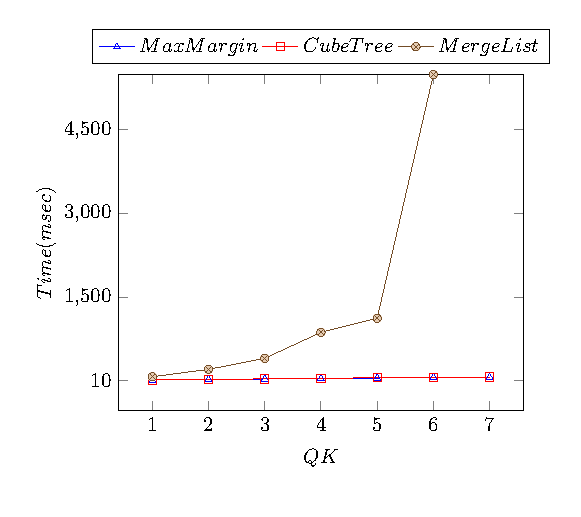
\includegraphics[width=1.5in,height=1.5in]{RQK-T}
    }
    \subfigure[] { \label{RQKb}
    \includegraphics[width=1.5in,height=1.5in]{RQK-R}
    }
\caption{Varying the factor QK}
\label{F9}
\end{figure}

\begin{figure}[h] \centering
    \subfigure[] { \label{RTSa}
    \includegraphics[width=1.5in,height=1.5in]{RTS-T}
    }
    \subfigure[] { \label{RTSb}
    \includegraphics[width=1.5in,height=1.5in]{RTS-R}
    }
\caption{Varying the factor TS}
\label{F10}
\end{figure}

Each object of Geographic Names is a 2D location associated with a set of items describing it (e.g., a geographic name like Locate). We use the \textit{feature class} (e.g., School and Hospital) as the keyword. Since there is only one single feature class associated with each object, which is different from our assumption that each object is associated with several keywords. To address this problem, we associate object o with keywords obtained by aggregating the feature class of all objects whose distance to o within a given threshold. Finally, we obtain 20,694 objects in total as shown in Table \ref{T5}. And we assign an integer number (e.g., 1,2,3,4,5) randomly for it as the level information, an integer number ranges from 1 to 100 as the cost of o.

Since factors of TK, DS and KD are fixed for CA dataset. We study the effect of QK and TS on real dataset. Figs. \ref{F9} and \ref{F10} show the experiment results of QK and TS, respectively. As can be observed from Fig. \ref{F9}a that MergeList runs out of memory when QK takes the value of 7, and both CubeTree and MaxMargin almost not be affected by QK, which is consistent with the observations in Fig. \ref{F6}a. Fig. \ref{F9}b shows that the solution of MaxMargin extremely approaches to optimal solution. However, the accuracy of CubeTree is unstable. Fig. \ref{F10} shows the performance of our algorithms when we vary TS from 0.1 to 0.7, as shown in Fig. \ref{F10}, the performance is consistent with the observations in Fig. \ref{F8}.

From the comprehensive experiments on both synthetic and real-life datasets, we can see that, both CubeTree and MaxMargin run much faster than the exact algorithm MergeList. CubeTree runs slightly faster than MaxMargin, however, MaxMargin with better performance than CubeTree in terms of accuracy and stability of approximation ratio. 